\documentclass[12pt]{report}
\usepackage[utf8]{inputenc}
\usepackage[russian]{babel}
%\usepackage[14pt]{extsizes}
\usepackage{listings}

% Для листинга кода:
\lstset{ %
language=python,                 % выбор языка для подсветки 
basicstyle=\small\sffamily, % размер и начертание шрифта для подсветки кода
numbers=left,               % где поставить нумерацию строк (слева\справа)
numberstyle=\tiny,           % размер шрифта для номеров строк
stepnumber=1,                   % размер шага между двумя номерами строк
numbersep=5pt,                % как далеко отстоят номера строк от подсвечиваемого кода
showspaces=false,            % показывать или нет пробелы специальными отступами
showstringspaces=false,      % показывать или нет пробелы в строках
showtabs=false,             % показывать или нет табуляцию в строках            
tabsize=2,                 % размер табуляции по умолчанию равен 2 пробелам
captionpos=t,              % позиция заголовка вверху [t] или внизу [b] 
breaklines=true,           % автоматически переносить строки (да\нет)
breakatwhitespace=false, % переносить строки только если есть пробел
escapeinside={\#*}{*)}   % если нужно добавить комментарии в коде
}

% Для измененных титулов глав:
\usepackage{titlesec, blindtext, color} % подключаем нужные пакеты
\definecolor{gray75}{gray}{0.75} % определяем цвет
\newcommand{\hsp}{\hspace{20pt}} % длина линии в 20pt
% titleformat определяет стиль
\titleformat{\chapter}[hang]{\Huge\bfseries}{\thechapter\hsp\textcolor{gray75}{|}\hsp}{0pt}{\Huge\bfseries}

%отступы по краям
\usepackage{geometry}
\geometry{verbose, a4paper,tmargin=2cm, bmargin=2cm, rmargin=1.5cm, lmargin = 3cm}
% межстрочный интервал
\usepackage{setspace}
\onehalfspacing
\usepackage{float}
% plot
\usepackage{pgfplots}
\usepackage{filecontents}
\usepackage{amsmath}
\usepackage{tikz,pgfplots}
\usetikzlibrary{datavisualization}
\usetikzlibrary{datavisualization.formats.functions}

\usepackage{graphicx}
\graphicspath{{src/}}
\DeclareGraphicsExtensions{.pdf,.png,.jpg}
\usepackage{amsmath}
\usepackage{geometry}
\geometry{verbose, a4paper,tmargin=2cm, bmargin=2cm, rmargin=1.5cm, lmargin = 3cm}
\usepackage{indentfirst}
\setlength{\parindent}{1.4cm}

\usepackage{titlesec}
\titlespacing{\chapter}{0pt}{12pt plus 4pt minus 2pt}{0pt}

\begin{filecontents}{timeHash.dat}
	100000 5.187925
	500000 30.5863
	700000 41.655
	1000000 58.1547
\end{filecontents}

\begin{document}
%\def\chaptername{} % убирает "Глава"
\begin{titlepage}
	\centering
	{\scshape\LARGE МГТУ им. Баумана \par}
	\vspace{3cm}
	{\scshape\Large Рубежный контроль №1\par}
	\vspace{0.5cm}	
	{\scshape\Large По курсу: "Анализ алгоритмов"\par}
	\vspace{1.5cm}
	{\huge\bfseries Поиск двоек, троек, четверок пользователей, размечавших один параграф\par}
	\vspace{2cm}
	\Large Работу выполнила: Маковская Яна, ИУ7-54\par
	\vspace{0.5cm}
	\Large Преподаватели:  Волкова Л.Л., Строганов Ю.В.\par

	\vfill
	\large \textit {Москва, 2019} \par
\end{titlepage}

\tableofcontents

\newpage
\chapter*{Задание}
\addcontentsline{toc}{chapter}{Введение}

Задание существует таблица, содержащая следующие сущности: phrase-id, user-id, paragraph-id (Рис. \ref{exp}). Необходимо выбрать все двойки или тройки или четверки пользователей, которые работали над одним параграфом.

\begin{figure}[h!]
	\begin{center}
		\begin{tabular}{|c c c|} 
			\hline
			phrase-id  & user-id & paragraph-id\\ [0.5ex] 
			\hline\hline
			1 & 41 & 29  \\
			\hline
			2 & 44 & 37\\
			\hline
			... & ... & ... \\
			\hline
		\end{tabular}
	\end{center}
	\caption{Таблица исходных данных}
	\label{exp}
\end{figure}

Задачи данной лабораторной работы:
\begin{itemize}
	\item Разработать алгоритм решения задачи;
\end{itemize}


\chapter{Аналитическая часть}
Для решения данной задачи было решено использовать сортировку, а затем вычленение пользователей, разметивших один и тот же абзац.

\section{Сортировка и нахождение групп} 
Для данной программы было решено использовать метод sorted из стандартной библиотеки Python. Отсортируем нашу исходную таблицу по параграфам, после чего можно будет перейти к поиску двоек, троек или четверок пользователей, разметивших один и тот же абзац. После сортировки таблицы по всей таблице циклом при помощи переменной-счетчика будут найдены необходимые группы пользователей.

\chapter{Конструкторская часть}
В данном разделе будут рассмотрены основные требования к программе.

\section{Требования к программе}
\textbf{Требования к вводу:}
\begin{itemize}
	\item Заранее известно сколько сущностей находится в таблице;
	\item cущности располагаются в таблице с небольшим разбросом.
\end{itemize}

\textbf{Требования к программе:}
\begin{itemize}
	\item Алгоритм возвращает все двойки, тройки и четверки пользователей, работавших над одним параграфом.
\end{itemize}


\section*{Вывод}
\addcontentsline{toc}{section}{Вывод}
В данном разделе были рассмотрены требования к программе.


\chapter{Технологическая часть}

\section{Выбор ЯП}
В качестве языка программирования был выбран python.
\section{Сведения о модулях программы}
Программа состоит из:
\begin{itemize}
	\item main.py- главный файл программы, в котором располагается точка входа в программу.
	\item generator.py - файл, генерирующий исходную таблицу.
\end{itemize}
\section{Листинг кода алгоритмов}
В данном разделе будут приведены листинги кода решения (Листинг \ref{brute}) и генератора таблицы (Листинг \ref{hash})
\begin{lstlisting}[label=brute,caption = Поиск, language = python]

def main():

    file = open("table.txt", 'r')
    table = [line.split() for line in file]
    for i in range(len(table)):
        table[i] = [int(x) for x in table[i]]

    # 0: phrase; 1: user; 2: paragraph;
    table = sorted(table, key=lambda line: line[2])

    cnt = 0
    prev_paragraph = 1
    for i in range(len(table)):
        paragraph = table[i][2]
        if paragraph == prev_paragraph:
            cnt += 1
        else:
            if 1 < cnt < 5:
                if cnt == 2:
                    print("Двойка ", end='')
                elif cnt == 3:
                    print("Тройка ", end='')
                elif cnt == 4:
                    print("Четверка ", end='')
                print("пользователей (", end='')

                for j in range(cnt):
                    print(table[i - cnt + j][1], end='')
                    if j != cnt - 1:
                        print(',', end='')
                print(') размечала параграф номер', table[i][2])

            cnt = 0
        prev_paragraph = paragraph
}
\end{lstlisting}

\begin{lstlisting}[label=hash,caption = Генератор, language = python]

import random

def main():
    file = open("table.txt", 'w')
    lines = 1000
    for i in range(1, lines + 1):

        phrase_id = i
        user_id = random.randint(1, 100)
        paragraph_id = random.randint(1, 100)
        file.write(str(phrase_id) + ' ' + str(user_id) + ' ' + str(paragraph_id) + '\n')
    file.close()
} 
\end{lstlisting}
\section*{Вывод}
\addcontentsline{toc}{section}{Вывод}
В данном разделе были рассмотрены основные сведения о модулях программы и листинг кода алгоритмов.

\chapter{Исследовательская часть}
В даннном разделе будут приведены результаты работы алгоритма.

\section{Результаты работы алгоритма}
Пример результата изображен на рисунке 4.1. 

\begin{figure}[ht!]
\center{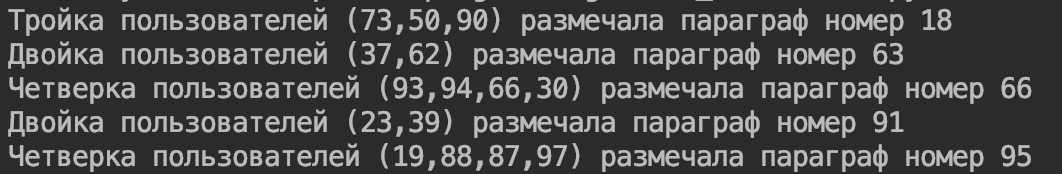
\includegraphics[scale=0.45]{result.png}}
\caption{Результат выполнения программы}
\end{figure}

\section{Выводы исследовательского раздела}
Программа работает корректно, выполнены все требования, поставленные для программного обеспечения.

\chapter*{Заключение}
\addcontentsline{toc}{chapter}{Заключение}
В ходе рубежного контроля был разработан алгоритм для решения поставленной задачи

\addcontentsline{toc}{chapter}{Список литературы}
\begin{thebibliography}{3}
	\bibitem{diskr} Кормен, Т., Лейзерсон, Ч., Ривест, Р., Штайн, К. Глава 11. Хеш-таблицы. // Алгоритмы: построение и анализ = Introduction to Algorithms / Под ред. И. В. Красикова. — 2-е изд. — М.: Вильямс, 2005. — 1296 с. — ISBN 5-8459-0857-4.
	\bibitem{commi2} Брюс Шнайер. Прикладная криптография. Протоколы, алгоритмы, исходные тексты на языке Си. — М.: Триумф, 2002. — ISBN 5-89392-055-4.
	\bibitem{commi} Дональд Кнут. Искусство программирования. Том 3. Сортировка и поиск = The Art of Computer Programming, vol.3. Sorting and Searching. — 2-е издание. — М.: «Вильямс», 2007. — С. 824. — ISBN 0-201-89685-0.
\end{thebibliography}

\end{document}

